\chapter{Core Knowledge}\label{cap:planificación}

\section{Introduction}

There are currently numerous techniques used in artificial intelligence. These not only come from physics or mathematics, but are also closely related to economics and computer science. Such is the catalog of possibilities available to us that it is often difficult to keep up to date, as new ideas emerge every day. Therefore, in order to obtain a better general understanding of this work, we will explain the principles of some of the methods or techniques used in the project, since understanding them will make it easier to follow the workflow. 
s
\section{Neural Networks}

If we look at the history of science and technology, we can observe that many advances are inspired by real biological systems. For example, a camera shares many similarities with the human eye. Another example is the processor, which consists of a large number of transistors connected to perform calculations. Neural networks are also part of this trend, as their structure is approximately based on biological neural networks. 

Neural networks are a type of machine learning model inspired by the human brain. They are designed to recognise patterns or relationships between data. This feature makes them the ideal type of model for images, language processing, or predictive modelling.

To fully comprehend this research, it is necessary to understand the following concepts.

\subsection{Relevant layers for this research}

There are numerous options available when selecting the appropriate layers for a neural network, each serving a distinct and well-defined purpose. Given the wide variability of existing architectures, this study will briefly describe the most influential layer types employed during the research, focusing on those that had the most significant impact on model performance and learning behavior.

\begin{itemize}
    \item \textbf{Dense}: Also known as fully connected, it is one of the simplest and best-known layers. Each neuron receives one input from each neuron in the previous layer and produces one output per neuron.
    \item \textbf{Convolutional 1D layers}: This is a layer used in neural networks to process sequential information, such as text, audio or genes. It allows one-dimensional convolution filters to be applied, thereby extracting relationships and patterns from the data. The output of a Conv1D layer is a feature map that captures the patterns extracted from the input data. These maps highlight local relationships in the sequence, such as recurring motifs or trends. However, one potential drawback of stacking many convolutional layers is that the original low-level information can become increasingly abstract or diluted. While deeper layers tend to capture more complex features, they may also lose fine-grained details present in the raw data.
\end{itemize}

\subsection{Regularization methods}

Regularisation is applied to machine learning models to prevent overfitting, which occurs when they learn the training data too well, including noise and outliers. This results in poorer generalisation when faced with new data.

Some examples include:
\begin{itemize}
    \item \textbf{L1 and L2 regularization}: Also known as Lasso (L1) and Ridge (L2) regularization, these techniques help prevent the model's weights from becoming too large. L1 Regularization encourages sparsity by driving less relevant weights to zero, effectively performing feature selection. L2 Regularization penalizes large weights more smoothly, distributing the error and promoting generalization.
    \item \textbf{Dropout}: This layer allows some neurons to be randomly reset to zero. This prevents the network from becoming overly dependent on a single neuron, thus avoiding overfitting.
    \item \textbf{Spatial dropout 1D}: This is an adaptation of dropout to networks in which convolutional layers are applied, so that the dimension of spatial dropout depends on the dimension of the convolutional layer, in this case 1.
    \item \textbf{Batch normalization}: Used to standardise the input to the layers, it reduces the impact of weight initialisation. It is very important to apply this layer before the activation function and not afterwards.
    \item \textbf{Max pooling}: It allows you to reduce the dimensionality of feature maps by selecting the maximum available using a sliding window.
\end{itemize}



\section{Predictions trees}

Decision trees are one of the most widely used types of machine learning algorithms, due not only to their great predictive power but also to their ease of interpretation, both in classification and regression tasks. The idea behind this algorithm is to divide the dataset into increasingly smaller subsets.

One of the main advantages is the interpretability they offer, without the need for any type of complex preprocessing or scaling. This makes them widely used in domains where understanding the reason behind each decision is important, such as biology or chemistry.

However, they do have disadvantages. For example, they are prone to overfitting, although there are techniques such as a posteriori pruning, maximum depth or minimum number of examples per leaf, to avoid this. But undoubtedly, the main drawback is that they are unable to generalise correctly when the test data falls outside the training domain.

The main types of tree algorithms include:

\begin{itemize}
    \item \textbf{CART}: It is a foundational decision tree algorithm, used for regression or classification tasks. It uses the Gini index or MSE to divide the data into different subsets, depending on whether it is a classification or regression problem.
    \item \textbf{RandomForest}: It is an ensemble learning method \footnote{Algorithms that combine several models, usually of the same type, produce an output based on all of them, applying techniques such as average voting.} used for both classification and regression tasks. It builds upon decision trees by combining multiple trees, which are independent, and aggregating their results to improve accuracy and reduce overfitting.
    \item \textbf{Gradient Boosted Trees}: This technique combines different decision trees, but unlike RandomForest, they are not independent. Each tree is trained with the aim of improving on those examples where the previous one failed. An example of this type of algorithm is XGBoost.
\end{itemize}

\section{SHAP values}

Based on Shapley values from cooperative game theory, SHAP is capable of measuring the contribution of a feature to a result, i.e., it quantifies the contribution of variables to the model output, both locally, a single example, and globally, the entire dataset. This allows us to determine which variables are most relevant in a prediction. 

The main advantage of SHAP over other explainability algorithms is that it provides a global view of the importance of the features in the entire dataset. In addition, thanks to its additive nature, it can be parallelised, as long as it is guaranteed that an example belongs to only one set, reducing computation times.

In addition, the implementation in Python \cite{shap} provides numerous graphs, thus facilitating the understanding of the data. For example:

\begin{itemize}
    \item \textbf{Summary plot}: This graph combines feature importance with their directional effect on the model's output, providing an intuitive representation of which variables are most influential, whether they contribute to an increase or decrease in predictions, and the range of input values that drive such behavior. The representation encompasses the entire dataset.
    
    \begin{figure}[H]
        \centering
        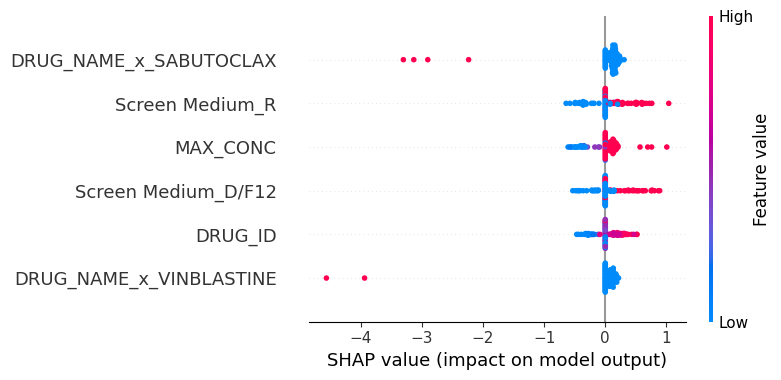
\includegraphics[width=1\textwidth]{figures/shap/shapValuesLittle.png}
        \caption{Example of SHAP values representation: Summary plot with 100 examples.}
        \label{fig:summaryPlot}
    \end{figure}

    \begin{itemize}
        \item Y-axis: The features sorted by relevance.
        \item X-axis: SHAP value. Impact on model output, a positive value show a higher predicton and vice versa.
        \item Dots: Each point represent a record of the dataset.
        \item Color: Indicate the feature value for that example.
    \end{itemize}
    

    \item \textbf{Force plot}: Used for local explainability. It provides the reasons why the prediction is higher or lower for an unique instance. In this type of graph, contrasting colors are used to show how each variable influences the prediction. Features that push the prediction higher are typically shown in red, while those that push it lower are shown in blue. This visualization helps to clearly distinguish between the variables that support and those that oppose the model's output for a specific instance.
    \begin{figure}[H]
        \centering
        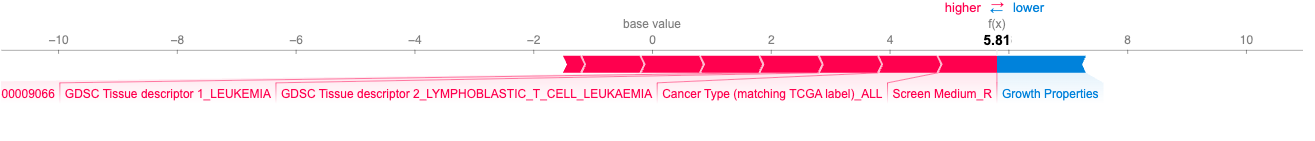
\includegraphics[width=1\textwidth]{figures/shap/force_plot.png}
        \caption{Example of SHAP values representation: Force plot with 100 examples.}
        \label{fig:forcePlot}
    \end{figure}

    Figure~\ref{fig:forcePlot} shows the variables that support increasing the value of the model output, while indicating that the Growth Properties variable is the only one that opposes this increase.

    \item \textbf{Dependence plot}: Used for global explainability. Show how a feature's value affect its SHAP value across the entire dataset helping to identify the relationship.
    \begin{figure}[H]
        \centering
        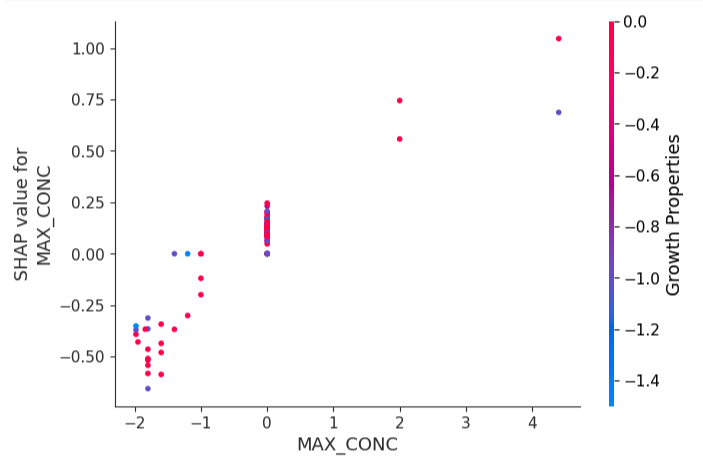
\includegraphics[width=1\textwidth]{figures/shap/depence_plot.png}
        \caption{Example of SHAP values representation: Dependence plot with 100 examples.}
        \label{fig:dependecePlot}
    \end{figure}

    \begin{itemize}
        \item Y-axis: The SHAP value for that variable, how much this feature contiributes to the model's output.
        \item X-axis: The value of the feature.
        \item Color: Indicate the second feature value.
    \end{itemize}

    In the example case shown in Figure~\ref{fig:dependecePlot}, it can be seen that as the MAX\_CONC variable decreases, it contributes less to a positive output, prompting a negative one.
\end{itemize}

